\documentclass{article}
\usepackage[dvipsnames]{xcolor}
\usepackage{indentfirst}
\usepackage[margin=1in]{geometry}
\usepackage[colorlinks=true,linkcolor=MidnightBlue]{hyperref}
\usepackage[shortlabels,inline]{enumitem}
\usepackage{amsmath}
\usepackage{amssymb}
\usepackage{amsthm}
\usepackage{tikz}
\usepackage{graphicx}

\usetikzlibrary{arrows.meta,positioning}

\setlist{nosep,itemsep=0.2ex}

\newtheorem{thm}{Theorem}
\theoremstyle{definition}
\newtheorem{defn}[thm]{Definition}
\theoremstyle{remark}
\newtheorem*{rmk}{Remark}

\newenvironment{aside}{\renewcommand{\thesection}{(\textit{\arabic{section}})}\renewcommand{\thesubsection}{(\textit{\arabic{section}.\arabic{subsection}})}}{\renewcommand{\thesection}{\arabic{section}}\renewcommand{\thesubsection}{\arabic{section}.\arabic{subsection}}}

\title{Drawing hyperbolic tilings}
\author{Evin}
%\date{}

\begin{document}
\maketitle

\section{Introduction}
On the fourth problem set of Hyperbolic Geometry and Mathematical Art, question 3 asked for making different tilings of the hyperbolic plane. I thought, ``wouldn't it be nice to have a program to do that automatically?'' Unfortunately, it was at around 11 PM on Thursday that I had this thought, and the show and tell would be tomorrow. So the next day I woke up early and spent an hour before breakfast building a sloppy prototype to share.

Afterwards I ended up spending the weekend completely redesigning the generator into something that's clean, mathematically interesting, and good enough to publish. This document is about all of the math that goes into it.

\section{The hyperboloid model}
The Poincar\'e disk model is nice, but it's not the most well-suited for geometric computations. We like lines, but the Poincar\'e disk has circles. Also, the Poincar\'e disk heavily squishes hyperbolic space far from the origin, and this magnifies the effect of rounding errors. Fortunately there is another model that is amazing for doing computations in, so I just do all of the geometry in the hyperboloid model and then convert to the Poincar\'e disk for rendering.

This model is basically a twist on the model of spherical geometry being the geometry of a sphere. We embed the hyperbolic plane as a hyperboloid in some strange 3D space. This is very closely related to special relativity, so we will be using a lot of physics terminology.
\begin{defn}
    The \emph{Minkowski space} $\mathbb R^{2+1}$ is the vector space $\mathbb R^3$ with the dot product replaced by
    \[(x_1,y_1,t_1)\cdot(x_2,y_2,t_2)=t_1t_2-x_1x_2-y_1y_2.\]
\end{defn}

For a vector $v$, let $\Vert v\Vert$ denote the norm, or squared length. We calculate the length by $\Vert v\Vert=v\cdot v$, just like in Euclidean space. So our choice of dot product endows $\mathbb R^{2+1}$ with a geometry, which is the geometry of special relativity. In particular, we call our coordinates $x$, $y$, and $t$ because $x$ and $y$ act like spatial coordinates and $t$ acts like the time coordinate. Also, note that the length squared can be negative! We can split all of the vectors into three types based on the squared length.
\begin{defn}
    A vector $v\in\mathbb R^{2+1}$ is
    \begin{itemize}
        \item \emph{timelike} if $\Vert v\Vert>0$,
        \item \emph{lightlike} if $\Vert v\Vert=0$,
        \item \emph{spacelike} if $\Vert v\Vert<0$.
    \end{itemize}
\end{defn}

Now the ``unit sphere'' $S$ in this space is the set of all vectors $v$ with $\Vert v\Vert=1$, which geometrically is a hyperboloid of two sheets. The future sheet $S_+$ is the sheet where everything has a positive time coordinate, and the past sheet $S_-$ is the sheet where everything has a negative time coordinate. The points in $S_+$ will be the points of our hyperbolic plane.

\subsection{Relation to other models}
The hyperboloid model is related to the Poincar\'e disk by stereographic projection. Let the south pole be the point $(0,0,-1)\in S_-$. Then projecting through the south pole onto $t=0$ gives the Poincar\'e disk model.

We can also project through the origin $(0,0,0)$ onto some plane parallel to the $x$-$y$ plane, then this will also give a bijection from $S_+$ into the interior of some disk. In fact, lines in this new model will become straight lines! This model is called the Beltrami-Klein model. However this model has a compromise: while lines become straight, angles are not preserved.

Another model that can be projected to either the Poincar\'e disk or the Beltrami-Klein disk is the hemisphere model. This takes place on the hemisphere defined by $x^2+y^2+t^2=1,t>0$. Projecting onto the $x$-$y$ plane through the north pole gives the Poincar\'e disk, and projecting along the $t$-direction gives the Beltrami-Klein model.

When we use the vertical projection that relates the hemisphere and Beltrami-Klein models, but instead apply it to the hyperboloid model instead, we get a model of hyperbolic geometry that uses the entire plane. This model is called the Gans model, and it has the unique property that straight lines in the Gans model are hyperbolas. 

\begin{rmk}
    I accidentally rediscovered the Gans model by directly changing the radial coordinate in the Poincar\'e disk when I was trying to solve the issue of things getting compressed near the boundary.
\end{rmk}

\subsection{Defining geometry}
We could define the geometry of the hyperboloid model by its relation to the Poincar\'e disk. In my opinion it's much more elegant to try to define the geometry by analogy with spherical geometry, and then leave the relation to the Poincar\'e disk as a theorem/``exercise to the reader.'' This is because the definition of hyperbolic geometry with this setup is really, really nice.

We know what points are, so now let's define lines. In spherical geometry, lines are great circles, which are basically just planes through the origin. This gives us the definition of line.
\begin{defn}
    A line in the hyperboloid model is the intersection of $S_+$ with a plane through the origin.
\end{defn}
For computational purposes, a plane through the origin has an equation of the form $\ell\cdot v=0$ for some vector $\ell$, and so we can represent a line by its ``normal vector'' $\ell$. Note that this is not unique. Also, we need a line to actually have points, and it turns out that the line will have points iff $\ell$ is spacelike.

Next, let's do angles. In spherical geometry, we can just calulate the angle between two lines by taking the angle between their planes. We can do the same thing here.
\begin{defn}
    Let $L$ and $K$ be two lines. Then the angle between them is
    \[\theta=\cos^{-1}\left(\frac{L\cdot K}{\sqrt{\Vert L\Vert\cdot\Vert K\Vert}}\right).\]
\end{defn}
\begin{rmk}
    Note that if we scale $\ell_1$, say, by a positive real number, then it represents the same line and the angle is unchanged. However, if we scale $\ell_1$ be a negative real number, then the angle gets replaced by the supplementary angle. So our vectors actually represent directed lines.
\end{rmk}

And then, we have distances. The distance from $P$ to $Q$ on $S_+$ can be determined as the length of the shortest path from $P$ to $Q$ staying on $S_+$, since we already know how to calculate distances in the ambient Minkowski space. This gives the following distance formula.
\begin{defn}
    Let $P$ and $Q$ be two points. Then the distance between them is
    \[\vert PQ\vert=\cosh^{-1}(-P\cdot Q).\]
\end{defn}

\subsection{Doing geometry}
The geometry of the hyperboloid model is defined by simple concepts in linear algebra, and this leads to computing stuff being very nice. For example, the line between two points $P$ and $Q$ is determined (up to scale) as the vector $v$ satisfying $v\cdot P=v\cdot Q=0$. This is like the usual cross product, so we introduce a cross product for Minkowski space.
\begin{defn}
    The \emph{cross product} of two vectors $(x_1,y_1,t_1),(x_2,y_2,t_2)\in\mathbb R^{2+1}$ is given by
    \[(x_1,y_1,t_1)\times(x_2,y_2,t_2)=(y_1t_2-y_2t_1,t_1x_2-t_2x_1,{\color{blue}y_1x_2-y_2x_1}).\]
\end{defn}
Note that the $t$-coordinate in {\color{blue}blue} has a sign change compared to the ordinary cross product, which is necessary to have all the properties we want.
\begin{rmk}
    This is a good time to give my ramble about what the cross product \emph{actually is}. There is a unique up to scale function $\varepsilon(u,v,w)$ of three vectors satisfying the following properties:
    \begin{itemize}
        \item \emph{multilinearity}: $\varepsilon(\alpha u,v,w)=\alpha\varepsilon(u,v,w)$ and $\varepsilon(u_1+u_2,v,w)=\varepsilon(u_1,v,w)+\varepsilon(u_2,v,w)$, and similarly for the other two arguments.
        \item \emph{antisymmetry}: swapping any two arguments negates $\varepsilon$.
    \end{itemize}

    $\varepsilon$ is basically a way to measure volumes, and note that this definition doesn't care about the dot product, so it will do the same thing regardless of whether the space is ordinary $\mathbb R^3$ or Minkowski $\mathbb R^{2+1}$ or whatever geometry. Now the cross product is basically a way to represent $\varepsilon$: we can define the cross product of $u$ and $v$ to be the unique vector $u\times v$ such that $\varepsilon(u,v,w)=(u\times v)\cdot w$. In Minkowski space we changed the dot product while keeping the same $\varepsilon$, thus the cross product must change.
\end{rmk}

Anyways, using the cross product, we know that $u\times v$ has zero dot product with both $u$ and $v$. In fact, this solves three problems at once!
\begin{thm}
    For two points $P$ and $Q$, the line through $P$ and $Q$ is $P\times Q$. For two lines $L$ and $K$, their intersection point is the unique scalar multiple of $L\times K$ that lies on $S_+$ (if $L\times K$ is timelike). For a point $P$ and line $L$, the line through $P$ perpendicular to $L$ is $P\times L$.
\end{thm}

\begin{rmk}
    This naturally invites us to think of how $L\times K$ relates to the geometric properties of $L$ and $K$. If $L\times K$ is timelike, then $L$ and $K$ intersect. If $L\times K$ is spacelike, then $L$ and $K$ don't intersect. When $L\times K$ is lightlike, this is when they almost intersect but don't. In the Poincar\'e disk they would appear to intersect on the boundary.
\end{rmk}

These already account for a lot of geometry we want to do. But for making tilings, there's another extremely important operation: reflecting an object across a line. Fortunately, this is also easy.
\begin{thm}
Given an object $X$ and line $L$, the reflection of $X$ across $L$ is
\[\sigma_L(X)=X-2\frac{X\cdot L}{L\cdot L}L.\]
\end{thm}
\begin{proof}
    We want to reflect $X$ over the plane perpendicular to $L$. Now consult the diagram.

    \begin{figure}[h]
        \centering
        \begin{tikzpicture}
            \draw[-{>[length=1mm,width=2mm]}] (0,0)--(5,0);
            \node[anchor=west] at (5,0) {$L$};
            \draw[-{>[length=1mm,width=2mm]}] (0,0)--(4,2);
            \node[anchor=west] at (4,2) {$X$};
            \draw[dashed,red] (4,2)--(4,0);
            \draw[-{>[length=1mm,width=2mm]},dashed,blue] (0,0)--(4,0);
            \node[anchor=north] at (4,0) {$v=\frac{X\cdot L}{L\cdot L}L$};
            \draw[Fuchsia] (0,3)--(0,-1);
            \node[anchor=north] at (0,-1) {$L^\perp$};
            \draw[dashed,blue] (4,2)--(-4,2);
            \draw[-{>[length=1mm,width=2mm]}] (0,0)--(-4,2);
            \node[anchor=east] at (-4,2) {$\sigma_L(X)$};
            \node[anchor=south] at (2,2) {$v$};
            \node[anchor=south] at (-2,2) {$v$};
        \end{tikzpicture}
    \end{figure}
\end{proof}

The tiling generator also uses one other construction. In the `Poly3' tiling, we need to compute a point equidistant from all three sides of a triangle. We call this point the \emph{incenter}. There's also a nice way to calculate the incenter, using barycentric coordinates.
\begin{defn}
    Let $A$, $B$, $C$ be points of $S_+$. A point $P\in S_+$ has \emph{barycentric coordinates} $[x:y:z]$ in triangle $\triangle ABC$ if $P$ is a scalar multiple of $xA+yB+zC$.
\end{defn}
These are called barycentric, because if we assign masses $x$ to $A$, $y$ to $B$, and $z$ to $C$ then $P$ will be the center of mass. Also note that if we scale $x$, $y$, and $z$ by the same constant, then $P$ doesn't change.
\begin{thm}
    The incenter of $\triangle ABC$ has barycentric coordinates
    \[[\sin \angle A:\sin \angle B:\sin \angle C].\]
\end{thm}
\begin{proof}
    Let $L$, $K$, and $M$ be norm $-1$ vectors representing sides $BC$, $AC$, and $AB$. Then the angle bisectors of $\angle A$ are given by $K\pm M$ and similarly for the other angles. Then the intersection of angle bisectors of $\angle A$ and $\angle B$ are
    \[(K\pm_1 M)\times (L\pm_2 M)=K\times L\pm_1 M\times K\pm_2 K\times M.\]
    We know that $K\times L$ is a multiple of $C$ with length $\sqrt{\Vert K\Vert\cdot \Vert L\Vert}\sin\angle C$. So $K\times L=\pm C\sin\angle C$ and similarly for the other products, so this expression is the point with barycentric coordinates $[\pm \sin \angle A:\pm\sin\angle B:\pm\sin\angle C]$ in $\triangle ABC$. The incenter must lie on every angle bisector, so it has this form. But the only choice of signs that yields a point inside $\triangle ABC$ is all positive (or all negative, which is equivalent). So the incenter is $[\sin \angle A:\sin \angle B:\sin \angle C]$.
\end{proof}
\begin{rmk}
    If you are familiar with barycentric coordinates in Euclidean geometry, this expression also works in the Euclidean case. It also works for spherical geometry.
\end{rmk}
\begin{rmk}
    I discovered that hyperbolic barycentric coordinates work accidentally, by computing the incenter this way. I couldn't figure out how to ensure the right choice of signs until realizing I could rewrite the expression as $\pm A\sin\angle A\pm B\sin\angle B\pm C\sin\angle C$ and then choose all positives. Then I noticed this was basically barycentric coordinates.
\end{rmk}

\begin{aside}
\subsection{The Darboux product}
An annoying thing about the Poincar\'e disk is that hyperbolic lines are circles. Actually, if we think hard enough about circles, then we can derive the hyperboloid model.

A circle can be written with an equation of the form
\[a(x^2+y^2)+bx+cy+d=0.\]
This form also allows lines as well, by setting $a=0$. So every hyperbolic line in the Poincar\'e disk can be put into this form.

We can view $(a,b,c,d)$ as a vector in $\mathbb R^4$. Similarly to the thing where representing a line in the hyperboloid model carries ``too much information,'' this representation does too. Scaling the vector yields the same circle but changes the vector. We choose to think of these vectors as ``weighted circles'' which have a mass given by $a$ in addition to their center and radius.

Recall that the power of a point $P$ with respect to a circle with radius $R$ and center $O$ is given by $OP^2-R^2$, and this has nice properties. Viewing a point as a circle with zero radius, the power of a point generalizes to the power between two weighted circles.
\begin{defn}
    Let $\Gamma$ be a weighted circle with mass $M_1$, center $O_1$, and radius $R_1$ and $\Delta$ be a weighted circle with mass $M_2$, center $O_2$, and radius $R_2$. Then the \emph{Darboux product} is given by
    \[\Gamma\cdot\Delta=M_1M_2(O_1O_2^2-R_1^2-R_2^2).\]
\end{defn}
\begin{thm}
    Suppose $\Gamma$ and $\Delta$ are weighted circles of masses $M_1$ and $M_2$ and radii $R_1$ and $R_2$ that intersect at an angle of $\theta$. Then
    \[\Gamma\cdot\Delta=2M_1M_2R_1R_2\cos\theta.\]
\end{thm}
\begin{proof}
    Let $O_1$ and $O_2$ be the centers of $\Gamma$ and $\Delta$, and let $P$ be one of the intersection points. Then $\theta=180^\circ-\angle O_1PO_2$, and then apply the law of cosines on $\triangle O_1PO_2$.
\end{proof}

\begin{rmk}
    Note that the squared length of a circle with mass $M$ and radius $R$ in for the Darboux product is $-2M^2R^2$. So this is basically the vector formula $u\cdot v= |u| |v| \cos\theta$ but using the Darboux product instead. This leads to a nice proof that inversion preserves angles.
\end{rmk}

If we compute everything we get the following formula.
\begin{thm}
    Let $\Gamma=(a_1,b_1,c_1,d_1)$ and $\Delta=(a_2,b_2,c_2,d_2)$ be weighted circles. Then
    \[\Gamma\cdot\Delta=d_1a_2+d_2a_1-\frac{b_1b_2}2-\frac{c_1c_2}2.\]
\end{thm}
\begin{rmk}
    This formula allows us to calculate the Darboux product for lines as well, by setting $a=0$.
\end{rmk}

So the Darboux product is also just a strange modified dot product, and we can use it to define the geometry on the space of circles. It turns out that it is equivalent by a change of variables to the dot product $(x_1,y_1,z_1,w_1)\cdot(x_2,y_2,z_2,w_2)=w_1w_2-x_1x_2-y_1y_2-z_1z_2$, which looks a lot like the Minkowski dot product.
\begin{defn}
    The space $\mathbb R^{3+1}$ is the space of weighted circles with the Darboux product as the dot product.
\end{defn}

Now it's time to relate all of this to hyperbolic geometry. Let $\Omega$ be the boundary of the disk, then the hyperbolic lines are exactly the weighted circles $\Gamma$ satisfying $\Gamma\cdot\Omega=0$. The Darboux product restricts to the space of hyperbolic lines to give it a geometry, and this geometry is exactly the geometry of $\mathbb R^{2+1}$.

This gives us the geometry of lines, but we want to look at the geometry of points. Fortunately, there's a good relationship between points and lines in this representation.
\begin{thm}
    For two points $P$ and $Q$ on the (Euclidean) plane, the space of weighted circles through $P$ and $Q$ is a plane through the origin in $\mathbb R^{3+1}$.
\end{thm}
We know that the hyperbolic lines through $P$ are the weighted circles through $P$ and its inverse. Thus they form a plane in $\mathbb R^{3+1}$ where everything is a hyperbolic line, so they form a plane in the space of hyperbolic lines. Then we can label $P$ by the vector perpendicular to this plane in $\mathbb R^{2+1}$.

\begin{rmk}
    This is an approach to representing hyperbolic things that I seriously considered. Then I realized it was equivalent to the hyperboloid.
\end{rmk}
\end{aside}

\section{Navigating the plane via group theory}
As you may have discovered on problem set 7, we can get from any triangle to any other triangle by repeatedly reflecting across hyperbolic lines. This suggests that we consider the group of symmetries of the tiling generated by reflections.

\begin{defn}
    Given a hyperbolic tiling $\mathcal T$, the \emph{Weyl group} $W(\mathcal T)$ is the group of all symmetries that can be obtained by repeated reflections across lines of the tiling.
\end{defn}

\begin{rmk}
    Note that the Weyl group might NOT contain all the symmetries of the tiling. For example, consider a tiling $\mathcal T$ by equilateral triangles with angles of $45^\circ$. Then the Weyl group is generated by reflections along sides of the triangles, but the full symmetry group also contains reflections about lines of symmetry of the triangles. In fact, for this example, we can split every equilateral triangle into six pieces by drawing in the lines of symmetry. This yields a tiling $\mathcal T'$ by triangles with angles $60^\circ$, $22.5^\circ$, and $90^\circ$. The Weyl group of this tiling is the full group of symmetries.
\end{rmk}

Now a computationally inconvenient fact about this definition is that there are infinitely many lines. Fotunately, we can generate the Weyl group with only finitely many reflections. Let's take a tiling and pick out favorite triangle in it.

\begin{figure}[h]
    \centering
    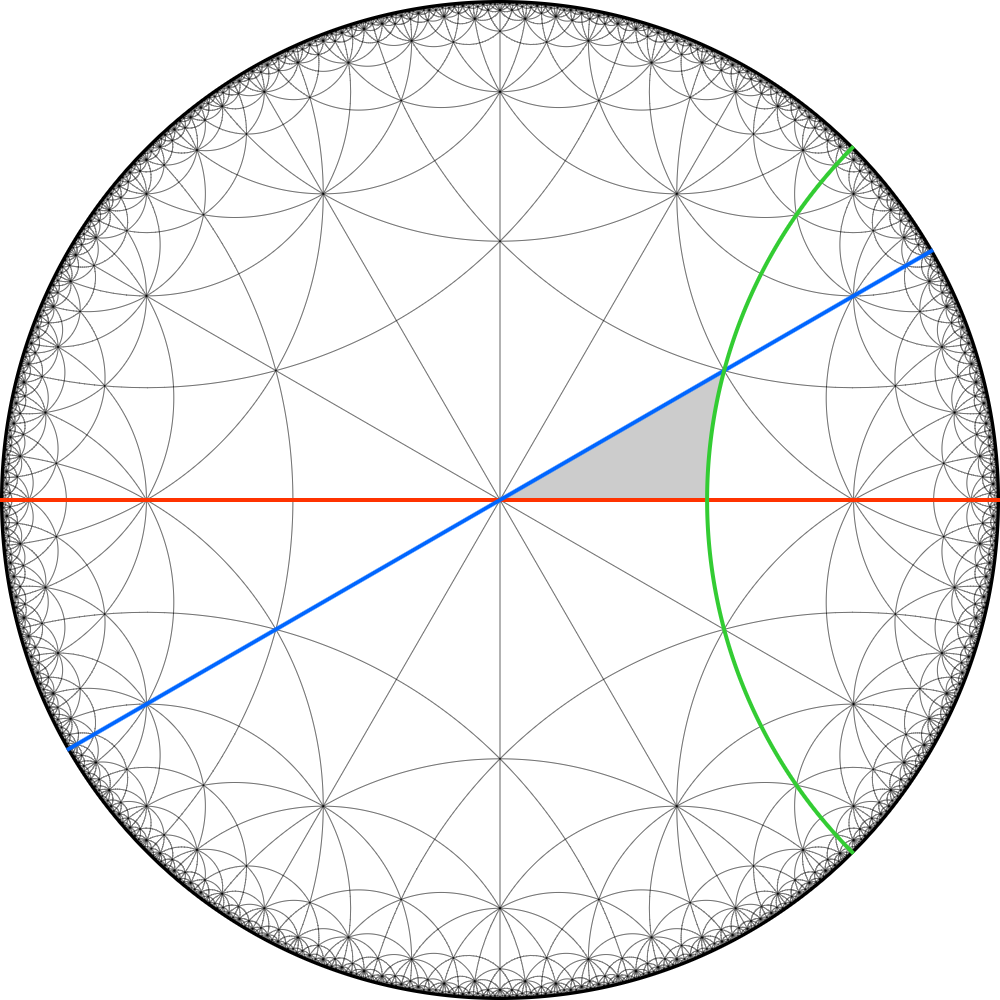
\includegraphics[width=0.6\textwidth]{trg_246.png}
\end{figure}

Let's label the three sides $a$, $b$, and $c$. By abusing notation, we will also let $a$, $b$, and $c$ denote the reflections about these three sides. You basically showed on problem set 9 that any element of the Weyl group can be obtained by composing $a$, $b$, and $c$. What are the relations between them?

\begin{thm}[Hard]
    Consider a tiling $\mathcal T$, where one triangle has sides $a$, $b$, and $c$. Suppose that the angle between $a$ and $b$ is $\frac\pi p$, the angle between $a$ and $c$ is $\frac\pi q$, and the angle between $b$ and $c$ is $\frac\pi r$. Then the Weyl group $W(\mathcal T)$ is generated by reflections about $a$, $b$, and $c$. Furthermore, every relation is a consequence of $a^2=b^2=c^2=(ab)^p=(ac)^q=(bc)^r=1$.
\end{thm}

The triangles in the tiling are nicely labeled by Weyl group elements, because it turns out that for any triangle $T'$ there is a unique Weyl group element that maps our starting triangle to $T'$. We know how to get from a triangle to its neighbors. So we can navigate the plane, provided we know how to do computations in the Weyl group.

\subsection{String rewriting}
Every element in the Weyl group can be written as a string in the letters $a$, $b$, and $c$ which represent the generators. We can treat the relations as rewrite rules that allow us to simplify a word while still representing the same element: for example, $a^2=1$ means that we can delete $aa$ anywhere in the word, and when $p=2$ we can delete $abab$ anywhere in the word. But sometimes we may need to apply these simplifcations in reverse. For example, suppose $p=3$. Then
\[baba\to babaababab\to ab\]
gives a simplification of $(ba)^2$ to $ab$, but one of the intermediate steps required making the string more complex. Can we modify this system so that we can always put anything in simplest form by only applying simplifying operations? Let's first define everything.

\begin{defn}
    A \emph{string rewriting system} is a set of \emph{rewrite rules} of the form $s\to t$ where $s$ and $t$ are strings. Rewriting a string by the rule $s\to t$ means replacing a substring $s$ with $t$.

    A rewriting system is \emph{terminating} if there is no string we can apply an infinite sequence of rewrites to. A rewriting system is \emph{confluent} if whenever a string $a$ can be rewritten to two strings $b$ and $c$, we can rewrite both $b$ and $c$ to the same string $d$. A rewriting system is \emph{strongly normalizing} if it is terminating and confluent.
\end{defn}

In particular, if we have a strongly normalizing rewrite system, we can always put strings in simplest form by repeatedly applying rewrites until we can't. Termination implies that we eventually finish, and confluence implies that we get the same result no matter what sequence we choose.

\begin{thm}[Folklore?]
    Given a hyperbolic tiling $\mathcal T$, there exists a strongly normalizing rewriting system for $W(\mathcal T)$. In fact, there exists such a system where every rewrite is ``downhill'' in the sense that it either decreases the length or keeps the length the same and makes the string lexicographically earlier.
\end{thm}

For example, let $\mathcal T$ be the tiling by equilateral triangles with angles of $36^\circ$. Then the Weyl group is generated by the reflections $a$, $b$, and $c$ satisfying $a^2=b^2=c^2=(ab)^5=(ac)^5=(bc)^5=1$. The rewriting system has 9 rules given by
\begin{align*}
    aa&\to 1\\
    bb&\to 1\\
    cc&\to 1\\
    babab&\to ababa\\
    cacac&\to acaca\\
    cbcbc&\to bcbcb\\
    cacabcbcb&\to acacabcbc\\
    cbcbacaca&\to bcbcbacac\\
    cacabcbcababa&\to acacabcbcabab
\end{align*}

These rules get pretty complicated! In fact, for many groups it will not even be possible to find such a rewriting system. So Weyl groups are quite special.

\subsection{Surfing and coloring}
So each triangle in the tiling is labeled with a string. We can move to the adjacent triangles by appending $a$, $b$, or $c$ to the end and putting it back into normal form, which correspond to reflecting about the three sides. This allows us to generate all the triangles. It also makes it easy to do so while avoiding duplication: whenever we make a simplification in the ``putting back into normal form'' part, we know that triangle will be a duplicate. So if we just want to generate a bunch of triangles, instead of doing the ``putting back into normal form'' we can just scan to see if a simplification applies and if so we toss it out.

The more exciting thing we can do with labels is to color the triangles! For example, the following simple coloring algorithms in the tiling generator yield nice results:
\begin{itemize}
    \item Triangle/Alternate: color by length mod 2.
    \item PolyA/Alternate: color by number of $c$s mod 2.
    \item PolyA/$D_n$: ???
\end{itemize}

The $D_n$ colorings have the most complicated rule. I stipulated the following requirements for the $D_n$ coloring:
\begin{itemize}
    \item Performing a type $a$ reflection leaves the coloring invariant.
    \item Every ``polygon'' centered at the intersection of a type $a$ line and type $b$ line is monochromatic.
\end{itemize}

Let's suppose further that in the relation $(ab)^p=(ac)^q=1$, that $p$ and $q$ are even. In terms of group theory, the first condition means that to find the color, we can pretend we have an extra relation $a=1$. Then we get the new set of relations $a=b^2=c^2=(bc)^r=1$.

This defines a simpler group, the \emph{dihedral group} (where the name $D_n$ for the coloring comes from!). This is the symmetry group of a regular $r$-gon. Let $D$ be this group, then basically what we are doing is taking a quotient $W(\mathcal T)\twoheadrightarrow D$. Basically, modular arithmetic but for groups.

Now let's look at the second condition. This requires that if we have a triangle, reflecting it over its $a$ or $b$ side preserves the color. Let $P$ be the subgroup of $D$ consisting of powers of $b$. Then define a \emph{left coset} of $P$ in $D$ to be a set of the form $gP:=\{gp\mid p\in P\}$ for some $g\in D$. The second condition is exactly saying that the coloring is constant on left cosets.

The two alternating colorings can also be described with this formulation. If you want to learn more about this take 18.701!
\end{document}
